%% ------ Packages ------ %%
% Related to the document setup:
\documentclass[12pt, a4paper]{extarticle}
\usepackage[a4paper, top = 2.4cm, bottom = 2.4 cm, right= 2.1cm, left= 2.1cm]{geometry}
\usepackage[english]{babel}
\renewcommand\familydefault{\sfdefault}
\usepackage{lmodern}
\usepackage{amsmath}
\usepackage{mathtools}
\usepackage{amsfonts}
\usepackage{amssymb}

\usepackage[T1]{fontenc}
\setlength\parindent{0pt}
\usepackage{multicol}
\usepackage{xspace}

\usepackage{tocloft}

% Colouring the references
\usepackage{hyperref}
\usepackage{cleveref}
\usepackage[dvipsnames]{xcolor}
\pagecolor{white}
\newcommand\myshade{85}
\colorlet{mylinkcolor}{violet}
\colorlet{mycitecolor}{YellowOrange}
\definecolor{myurlcolor}{rgb}{ 0, 0.4470, 0.6410}

\hypersetup{
  linkcolor  = mylinkcolor!\myshade!black,
  citecolor  = mycitecolor!\myshade!black,
  urlcolor   = myurlcolor!\myshade!black,
  colorlinks = true,
}

% Nomenclature
%\usepackage{nomencl}
%\makenomenclature
%%\renewcommand{\nomname}{List of symbols}
%\renewcommand{\nompreamble}{\noindent Definitions of the nomenclature}
%\newlength{\nomitemorigsep}
%\setlength{\nomitemorigsep}{\nomitemsep}
%\setlength{\nomitemsep}{-\itemsep}

% Section properties redefinitions
\makeatletter
\renewcommand\section{\@startsection {section}{1}{\z@}{3ex }{0.7ex } {\normalfont\large\bfseries}}
\renewcommand\subsection{\@startsection{subsection}{1}{\z@}{2ex }{0.1ex } {\normalfont \bfseries}}
\renewcommand\subsubsection{\@startsection{subsubsection}{3}{\z@}{-1.5ex\@plus -1ex \@minus -.2ex}{.5ex}{\normalfont}}
\makeatother

% Graphics interfaces:
\usepackage{graphicx}
\usepackage{tikz}
\tikzset{every picture/.style={line width=1pt}}
\usepackage{float}
\usepackage{subcaption} 
\usepackage[font=small,aboveskip=3pt, belowskip=-0pt]{caption}


% Headers and footers:
\usepackage{url}
\usepackage{footnote}
\usepackage{fancyhdr}
\pagestyle{fancy} 
\fancyhf{} 
\renewcommand{\headrulewidth}{0pt}
\newcommand{\mainmatter}{\clearpage \cfoot{\thepage\ of \pageref{LastPage}}
\setcounter{page}{1}
\pagenumbering{arabic}}
%\usepackage{comment}

\lfoot{\footnotesize \textcolor{Gray}{\thesistitle.}}
\rfoot{\footnotesize \textcolor{Gray}{\thesisauthor, \studentnumber. \thedate.}}
\fancyhfoffset{0pt}


% Sort the bibliography and add to the table of contents
\usepackage[sort]{cite}
\setlength\columnsep{15pt}
\usepackage[nottoc,numbib]{tocbibind}

% Redefine the \left and \right operators:
\let\originalleft\left
\let\originalright\right
\renewcommand{\left}{\mathopen{}\mathclose\bgroup\originalleft}
\renewcommand{\right}{\aftergroup\egroup\originalright}

% Redefine \eqref environment
\usepackage{letltxmacro}
\LetLtxMacro{\originaleqref}{\eqref}
\renewcommand{\eqref}{Equation~\originaleqref}

% Command definitions and macros:
\newcommand{\ic}{{\rm{i}}\xspace}
\renewcommand{\Re}{{\operatorname{Re}}\xspace}
\renewcommand{\Im}{{\operatorname{Im}}\xspace}

\newcommand{\Pulse}{{\mathcal{P}}\xspace}
\newcommand{\kmean}{{\langle k\rangle}\xspace}
\renewcommand{\k}{{\boldsymbol{k}}\xspace}
\newcommand{\kacc}{{\boldsymbol{k'}}\xspace}
\newcommand{\kin}{{k^{\rm in}}\xspace}
\newcommand{\kout}{{k^{\rm out}}\xspace}
\newcommand{\kinb}{{\boldsymbol{k^{\rm in}}}}
\newcommand{\koutb}{\boldsymbol{{k^{\rm out}}}}
\newcommand{\kinbi}{{\boldsymbol{k}_i^{\bf in}}}
\newcommand{\koutbj}{{\boldsymbol{k}_j^{\bf out}}}
\newcommand{\degree}{{\rm deg}\xspace}
\newcommand{\kmin}{k_{\text{min}}\xspace}
\newcommand{\kmax}{k_{\text{max}}\xspace}

\newcommand{\Sin}{{S^{\rm in}}\xspace}
\newcommand{\Sout}{{S^{\rm out}}\xspace}

\newcommand{\dtheta}{{\dot{\theta}}\xspace}

\newcommand{\permute}{{\digamma}\xspace}
\newcommand{\permuteinv}{{\digamma^{-1}}\xspace}

%\newcommand{\R}{{\rm I\!R}\xspace}
\newcommand{\R}{{\mathbb{R}}\xspace}
\renewcommand{\c}{{\mathbb{C}}\xspace}
\newcommand{\C}{\mathbb{C}_\circ}
\newcommand{\T}{{\mathbb{T}}\xspace}
\newcommand{\K}{{\mathbb{K}}\xspace}

\newcommand{\tp}{{t^{\prime}}\xspace}
\newcommand{\tpp}{{t^{\prime \prime}}\xspace}

\newcommand{\QIF}{{\textsl{QIF}}\xspace}
\newcommand{\PRC}{{\textsl{PRC}}\xspace}
\newcommand{\pdf}{{\textsl{pdf}}\xspace}
\newcommand{\MFR}{{\textsl{MFR}}\xspace}
\newcommand{\SNIC}{{\textsl{SNIC}}\xspace}
\newcommand{\PSR}{{\textsl{PSR}}\xspace}
\newcommand{\PSS}{{\textsl{PSS}}\xspace}
\newcommand{\CPW}{{\textsl{CPW}}\xspace}
\newcommand{\STDP}{{\textsl{STDP}}\xspace}
\newcommand{\ISI}{{\textsl{ISI}}\xspace}
\newcommand{\IP}{{\textsl{IP}}\xspace}



\def\matlab{\textsc{Matlab}\xspace}

% Author macros:
\newcommand{\thesistitle}{The dynamics of adaptive neuronal networks}
\newcommand{\thesissubtitle}{influence of topology on synchronisation }
\newcommand{\mywork}{{\textsl{Investigation:}}\xspace}

\newcommand{\thesisauthor}{Simon Aertssen} % Your name :) 
\newcommand{\studentnumber}{s181603}
\newcommand{\thedate}{February 1$^{\text{st}}$ 2021} 
\newcommand{\thesissupervisorI}{Erik Martens} 
\newcommand{\thesissupervisorII}{Poul Hjorth} 

\newcommand{\department}{DTU Compute}
\newcommand{\departmentdescriber}{Department of Applied Mathematics and Computer Science}
\newcommand{\addressI}{Richard Petersens Plads, Building 324}
\newcommand{\addressII}{2800 Kgs. Lyngby, DK}
\newcommand{\departmentwebsite}{www.compute.dtu.dk}


%% ------ Front page ------ %%

\begin{document}

\mainmatter

\section{Hebbian Learning}
\vspace{1mm}
\begin{quote}
\textsl{When an axon of cell A is near enough to excite a cell B and repeatedly or persistently takes part in firing it, some growth process or metabolic change takes places in one or both cells such that A's efficiency, as one of the cells firing B, is increased.}\cite{Hebb1949}
\end{quote}

\section{Spike Timing Dependant Plasticity}
Write about STDP, see the 'Postulates.pdf'. \\

With spike timing dependant plasticity we want to study how two neurons change their synaptic strength based on the time delay between spikes. When $\theta(t)_j > \pi$ we say that the neuron $\theta_j$ spikes at time $t$. 
Let us say that $\theta_i$ spikes at time $t_i$ and $\theta_j$ spikes at $t_j$. Taking the time difference $\Delta t_{ij}$ as $t_j - t_i$, we can say that when $\Delta t_{ij} > 0$ the spikes are correlated (there exists a temporally causal relation), and we can model an increase in synaptic strength of the connection $K_{ij}$ from $\theta_i$ to $\theta_j$. In the same fashion we can decrease $K_{ji}$ when $\Delta t_{ij} < 0$ as there is no causal relation. \\
The functions $W(t)$ that relate $\Delta t_{ij}$ to $\Delta K_{ij}$ are called \textsl{learning windows},  as they define a range in which $K_{ij}$ is able to adapt. When signals between neurons show a very large time difference (negative or positive) we do not expect them to be correlated. Because the learning windows are generally not symmetrical we can also expect an asymmetrical adjacency matrix.\\
Another characteristic is the integral over the learning window. A window with a negative integral directs synaptic strengths mostly towards inhibitory behaviour, and vice versa with a positive integral. An integral of zero would mean that both inhibitory and excitatory synapses are stimulated equally.\\

Now that we have a feeling of how \STDP works, we need to formulate the behaviour exactly. One by one, we will denote our ideas into mathematics.


\subsection{Biphasic learning windows}

\subsubsection{Kempter1999}
Following the notation in \cite{Kempter1999}, we will denote the spike train coming from each neuron $\theta_i$ as $S_i^{\rm out}(t) = \sum_{n} \delta (t-t_{i}^{n})$, where $t_{i}^{n}$ is the time that $\theta_i$ has fired. Similarly, we will denote the spike train coming into each neuron $\theta_i$ as $S_i^{\rm in}(t) = \sum_{f} \delta (t-t_{i}^{f})$. Now we can say that the synaptic strengths are adjusted as:
\begin{align}
\Delta K_{ij} &= \int_{t}^{t+\mathcal{T}} w^{\rm{out}} S_i^{\rm out}(\tau) + w^{\rm{in}} S_{j}^{\rm {in}}(\tau) \mathrm{d}\tau
+ \iint_{t}^{t+\mathcal{T}} W( \tau^\prime - \tau) S_{i}^{\rm out}(\tau) S_{j}^{\rm in}( \tau^\prime) \mathrm{d} \tau \mathrm{d} \tau^\prime
\label{eq:KempterSTDPFormulation1} \\
&= \sum_{t_i^{n}\in \mathcal{T}} w^{\mathrm{out}} + \sum_{t_{j}^{f} \in \mathcal{T}} w^{\mathrm{in}} + \sum_{t_{j}^{f}, t_i^{n} \in \mathcal{T}} W (t_{j}^{f}-t_i^{n} ) \label{eq:KempterSTDPFormulation2}
\end{align}
where \cite{Kempter1999} proposes the following learning window:
\begin{align}
W(t)_K = \alpha
\begin{cases}
\left[A_{p}\left(1-\frac{t}{\tilde{\tau}_{p}}\right)+A_{n}\left(1-\frac{t}{\tilde{\tau}_{n}}\right)\right] \cdot \exp \left( \frac{t}{\tau_{\rm syn}} \right) & \text{for } t \leq 0 \\
A_{p} \cdot \exp \left(-\frac{t}{\tau_{p}}\right) + A_{n} \cdot \exp \left(-\frac{t}{\tau_{n}} \right) & \text{for } t > 0
\end{cases} \label{eq:learningwindowKempter1999}
\end{align}
Here $t$ is the delay between presynaptic spike arrival and postsynaptic firing, $\alpha$ is a small learning parameter and all $\tau$ are time constants. Numerical values are usually  $\alpha = 0.05$, $\tau_{\rm syn} = 5$ ms, $\tau_{p} = 1$ ms, $\tau_{n} = 20$ ms and $A_p = 1$ and $A_{n} = -1$. $\tilde{\tau}_{p} \equiv \tau_{\rm syn} \tau_{p} / (\tau_{\rm syn} + \tau_{p})$ and $\tilde{\tau}_{n} \equiv \tau_{\rm syn} \tau_{n} / (\tau_{\rm syn} + \tau_{n})$. \\
$\int W(s)_K \mathrm{d}s = 2.56 \times 10^{-4}$.


\subsubsection{Song 2000}
The first formulation of \STDP as a mathematical model was in \cite{Song2000}. It is postulated without being concerned about the biological aspect too much. The synaptic strengths are simply updated as:
\begin{align}
\Delta K_{ij} &= K_{ij} \sum_{t_{j}^{f}, t_i^{n} \in \mathcal{T}} W (t_{j}^{f}-t_i^{n} ) \label{eq:SongSTDPFormulation}
\end{align}
The learning window is defined as a discontinuous function:
\begin{align}
W(t)_S =
\begin{cases}
A_{p} \cdot \exp \left(\frac{-t}{\tau_p}\right) & \text{for } s > 0 \\
A_{n} \cdot \exp \left(\frac{t}{\tau_n}\right)  & \text{for } s \leq 0
\end{cases} \label{eq:learningwindowKempter1999}
\end{align}
where we will use $A_p = 0.005$, $A_n = -0.00525$ and $\tau_p = \tau_n = 20$ ms. $\int W(s)_S \mathrm{d}s = -3.70 \times 10^{-4}$ so we expect the weights to be suppressed towards a negative value.

\begin{figure}[H]
\centering
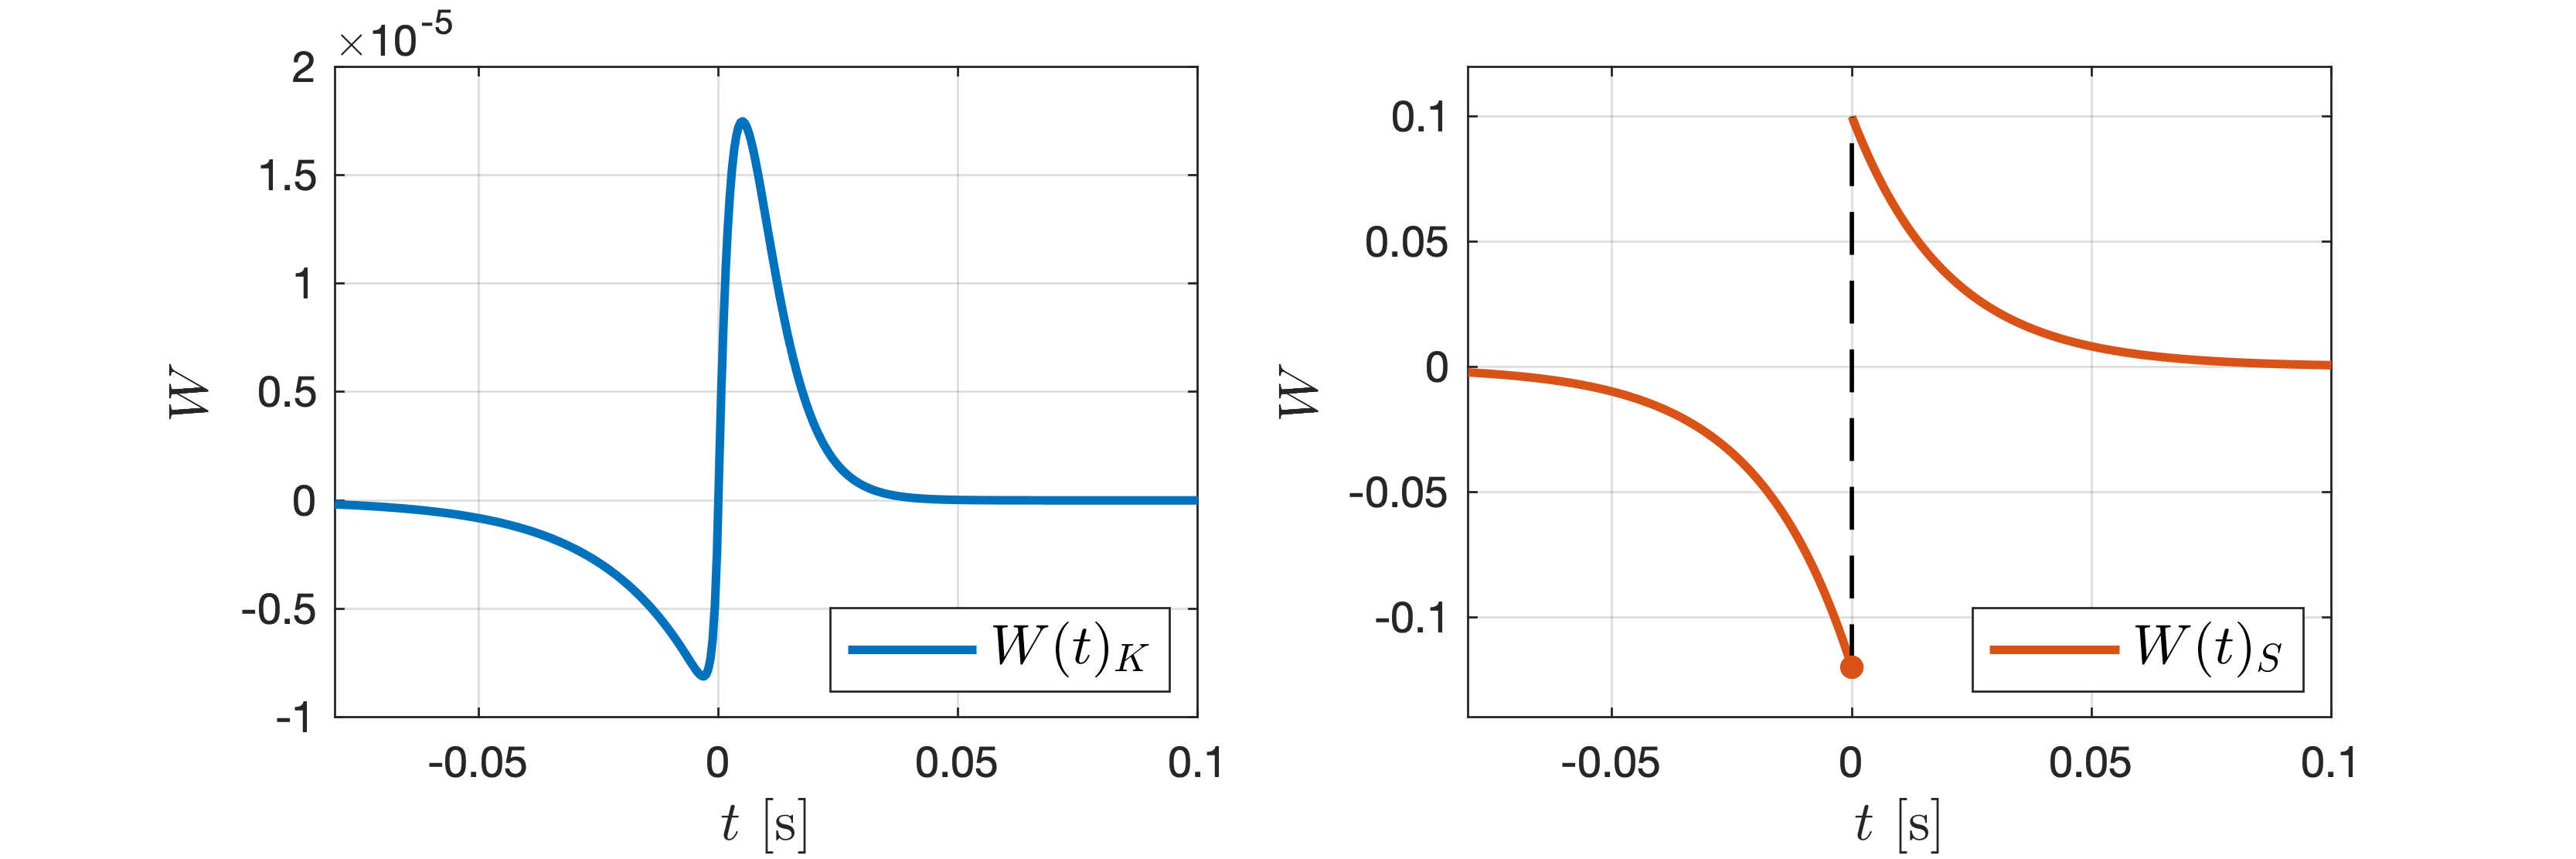
\includegraphics[width = \textwidth]{../Figures/LearningWindowsBiphasic.png}
\caption{Two different biphasic learning windows. We can see how in $W(t)_s$ a larger weight is put on the anti-Hebbian learning.}
\label{fig:LearningWindowsBiphasic}
\end{figure}


\subsection{Triphasic Learning windows}
Based off of neuronal actiity in the hippocmpus, biologically inspired triphasic windows have been developed. The papers describing the learning process are not specifying exactly how the weights are updated, as we have seen before there are a few options. We assume the change is simply:
\begin{align}
\Delta K_{ij} =  \sum_{t_{j}^{f}, t_i^{n} \in \mathcal{T}} W (t_{j}^{f}-t_i^{n} ) \label{eq:WaddingtonSTDPFormulation}
\end{align}
as there is no mention of other parameters.

\subsubsection{Chrol-Cannon 2012}
\begin{align}
W(t)_C = A_{p} \cdot \exp \left(\frac{-\left(t - 15 \right)^{2}}{ \tau_{p}}\right) - A_{n} \cdot \exp \left(\frac{-\left(t - 20\right)^{2}}{ \tau_{n}}\right)  \label{eq:learningwindowChrolCannon2012}
\end{align}
where $A_{p}=0.23$, $A_{n}=0.15$, $\tau_{p}=200$ and $\tau_n = 2000$. $\int W(s)_C \mathrm{d}s = -60.0 \times 10^{-4}$.

\subsubsection{Waddington 2014}
The learning window is then defined as:
\begin{align}
W(t)_W =  A \left[1-\frac{\left(t-\alpha\right)^{2}}{\alpha^{2}}\right] \cdot \exp \left(\frac{-\left|t - \alpha\right|}{\alpha}\right) \label{eq:learningwindowWaddington2014}
\end{align}
We will use $A = 0.1$ and $\alpha = 4.0$ ms . $\int W(s)_W \mathrm{d}s = -8.0 \times 10^{-4}$.

\begin{figure}[H]
\centering
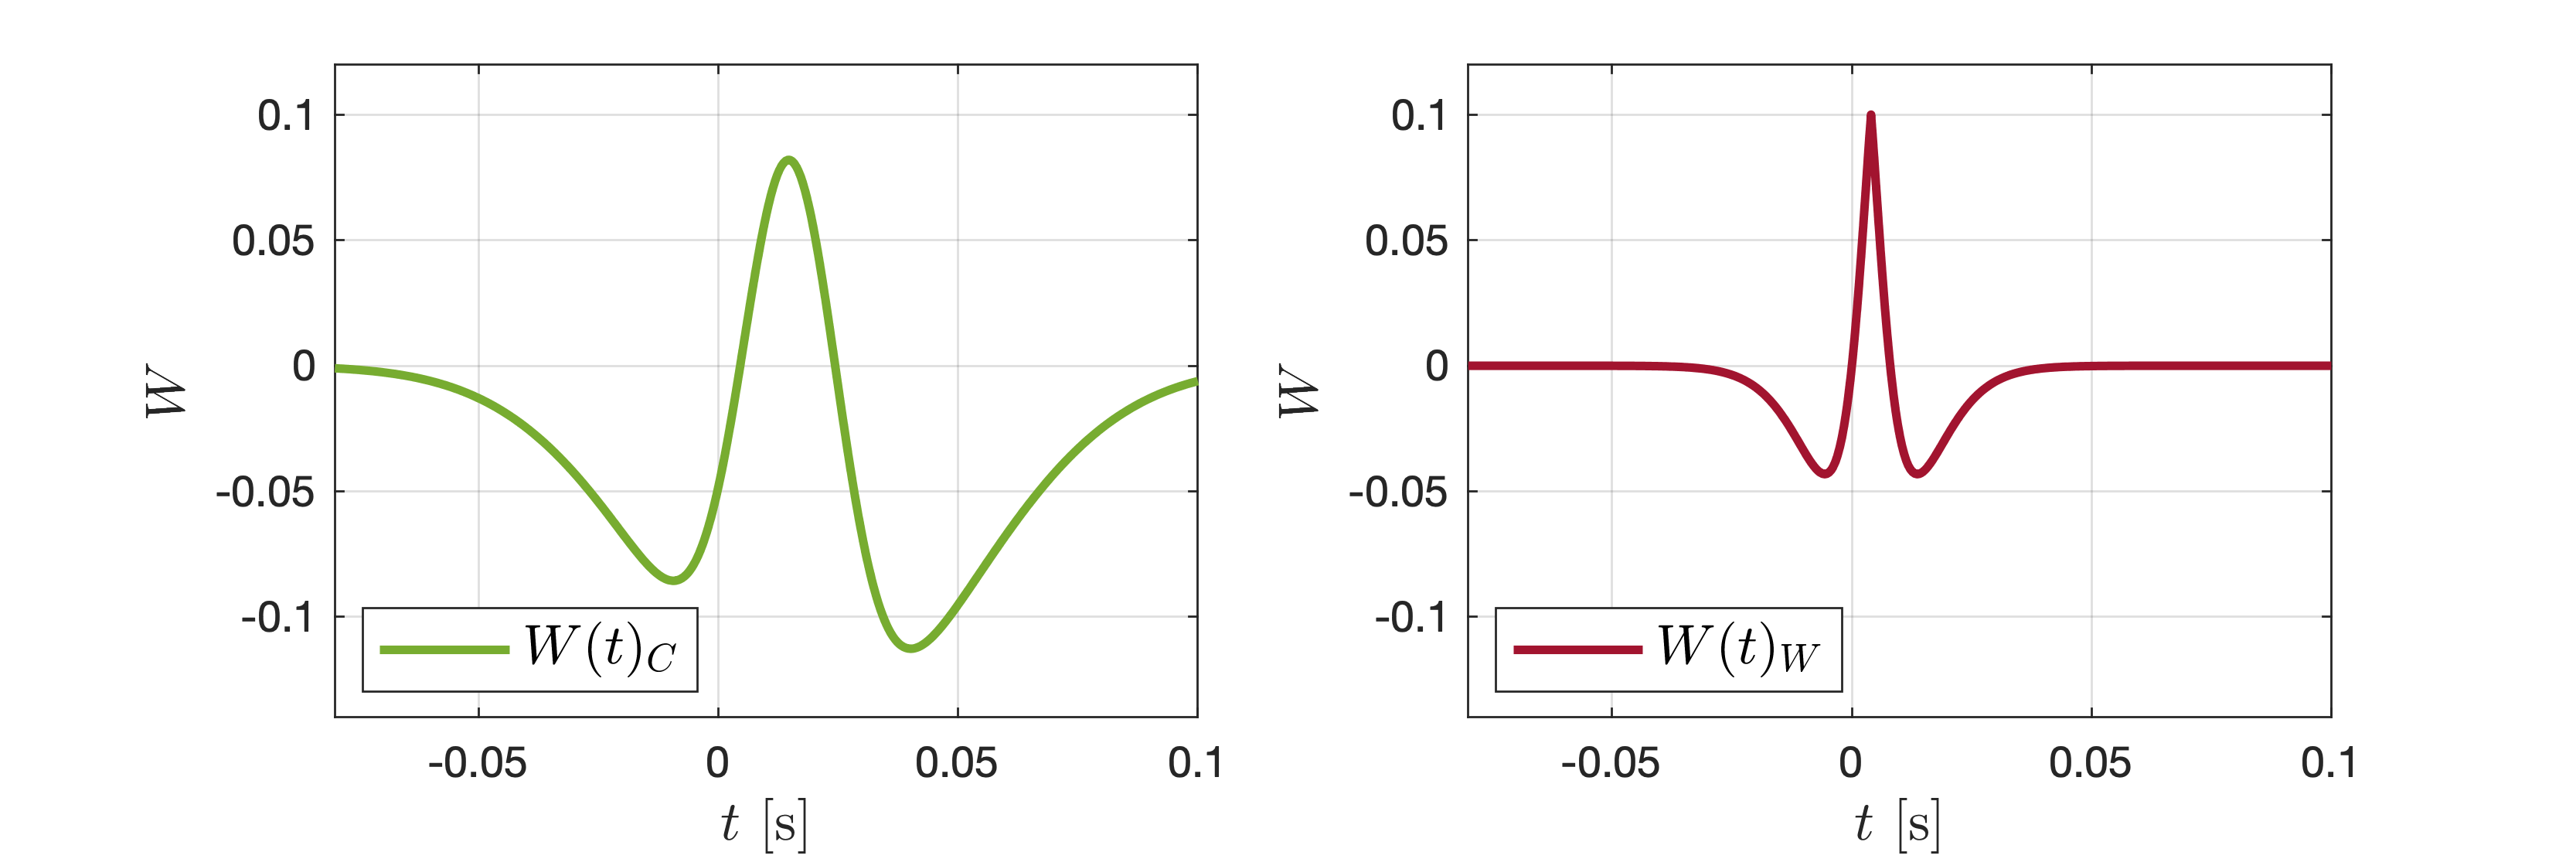
\includegraphics[width = \textwidth]{../Figures/LearningWindowsTriphasic.png}
\caption{The mean degree $\kmean$ evolves over time as a function of the spiking behaviour, just like we expect.}
\label{fig:LearningWindowsTriphasic}
\end{figure}


\subsection{Interpretation}
The learning windows generally have $W(t^{\ast}) = 0$ for $t^{\ast} > 0$. This means that no learning will take place when the delay between neuron spikes is exactly $t^{\ast} > 0$. The triphasic windows show two of those points.

\subsection{Results}
\begin{figure}[H]
\centering
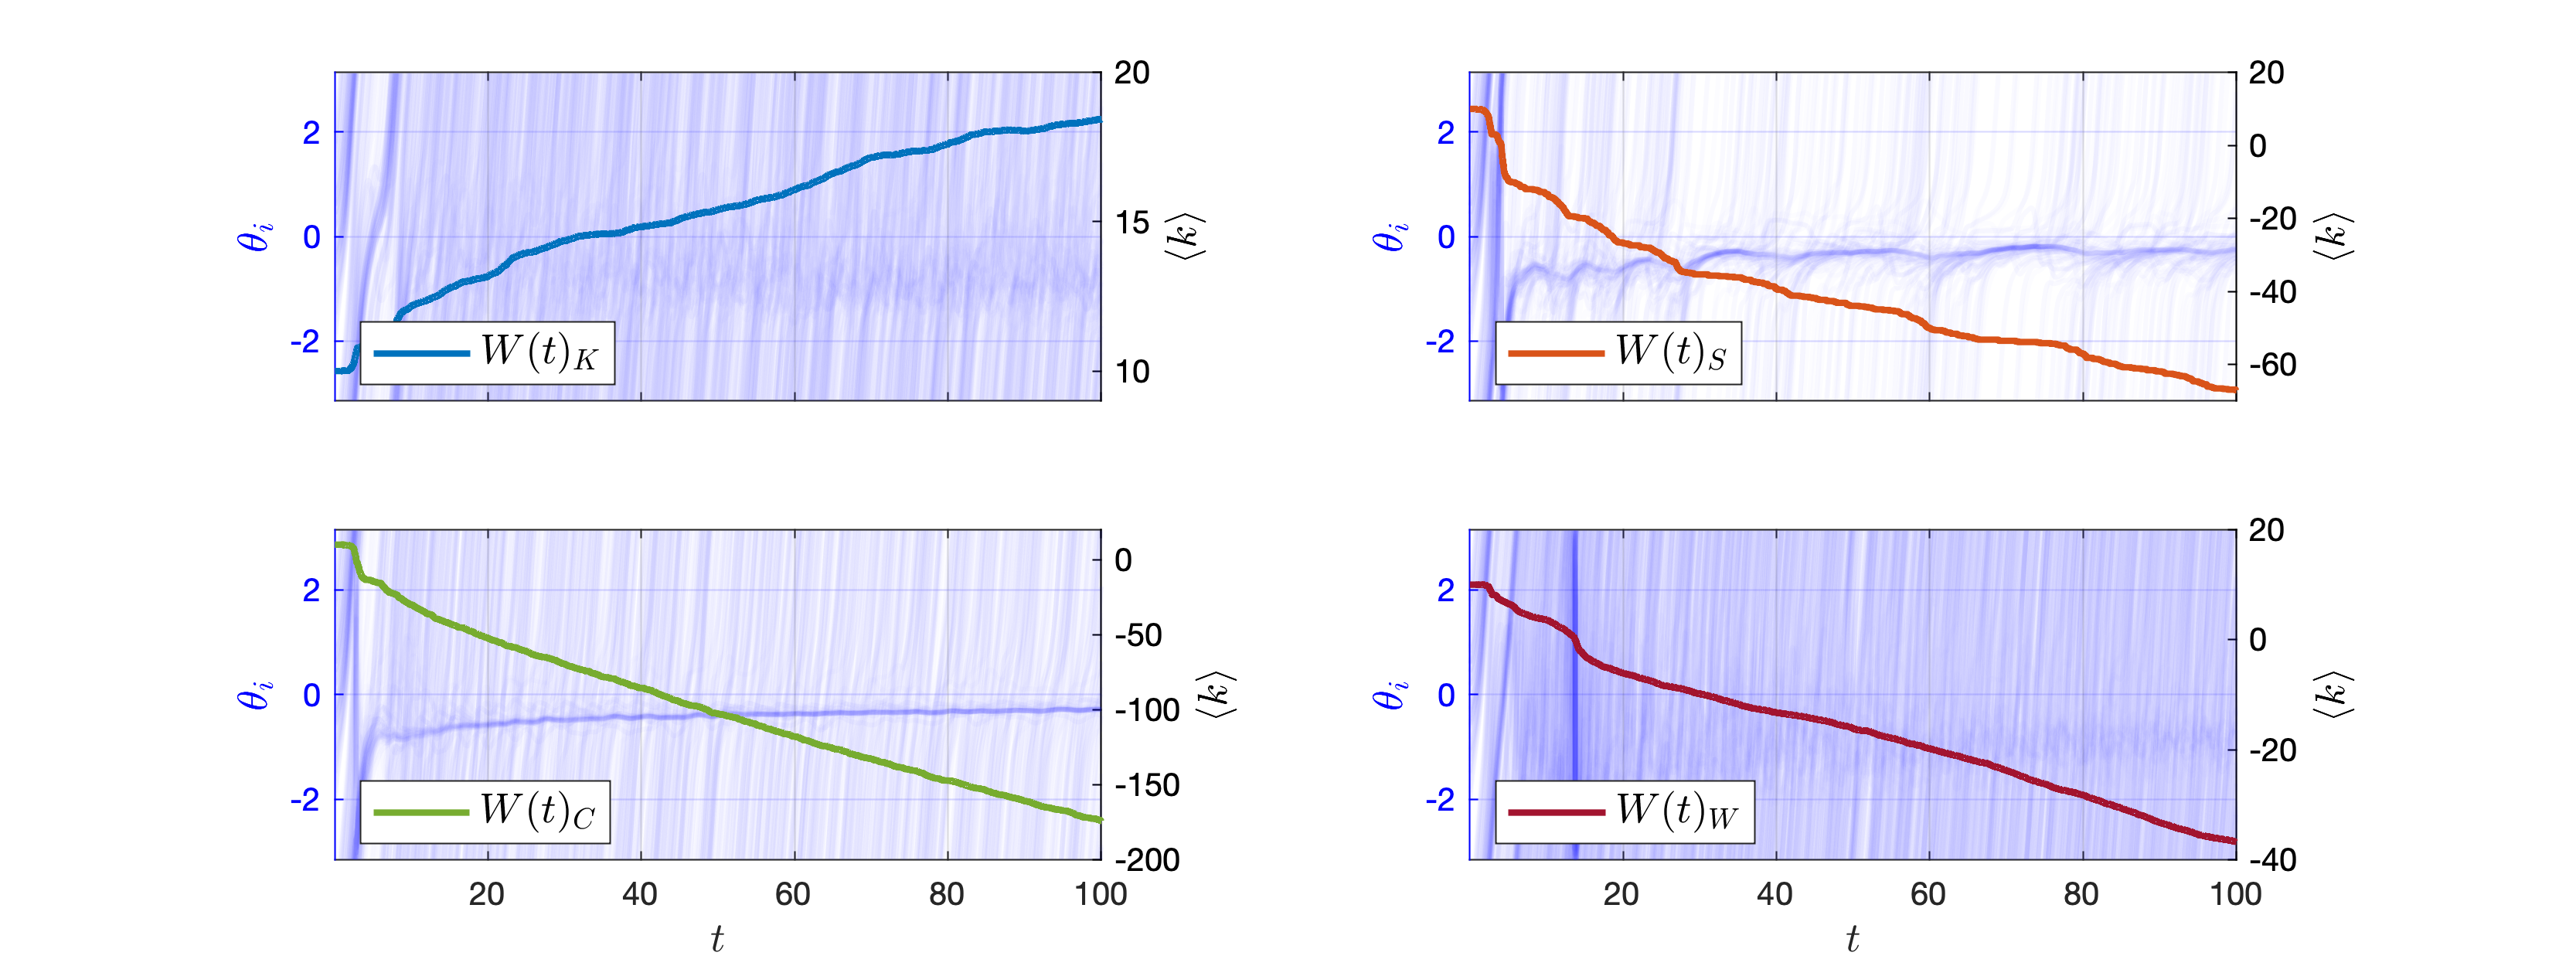
\includegraphics[width = \textwidth, trim={60 0 60 0}]{../Figures/LearningWithoutScaling.png}
\caption{Two different triphasic learning windows. We can see how in $W(t)_C$  a much higher penalty is given to signals that arrive too early or too late. The moments at which signals should peak also differ by about 10 ms.}
\label{fig:LearningWithoutScaling}
\end{figure}

\begin{figure}[H]
\centering
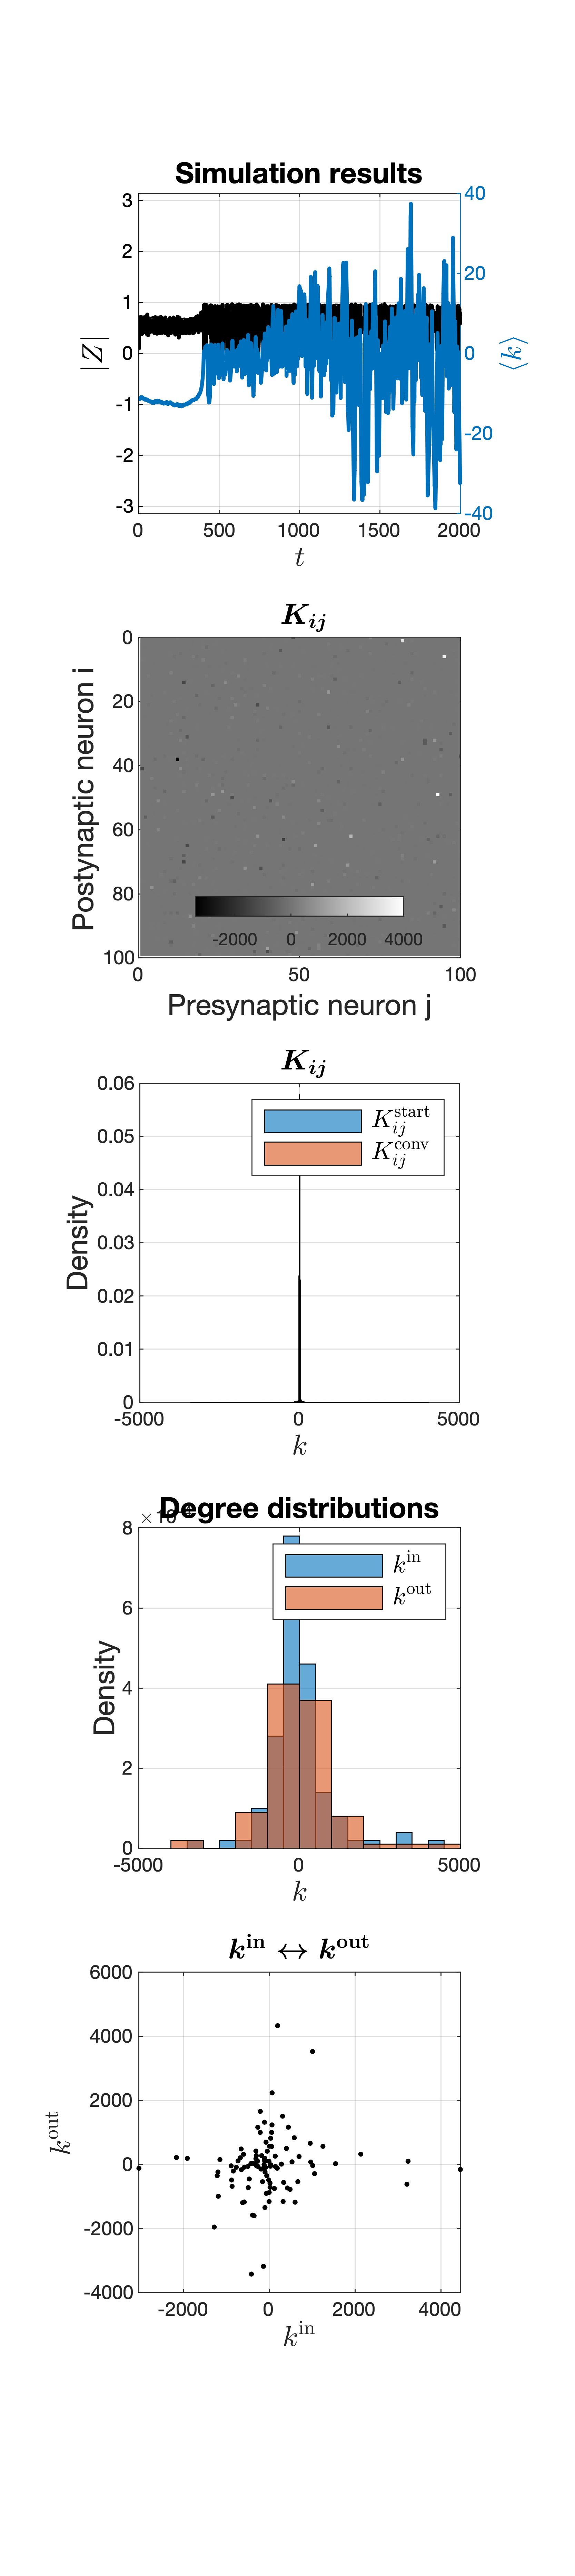
\includegraphics[width = 0.2\textheight]{../Figures/STDPbeforeIP.png}
\caption{Results from \STDP.}
\label{fig:STDPbeforeIP}
\end{figure}



\subsection{Synaptic scaling}
There is no upper or lower bound on the synapse strength. Also generally, connection strengths are nonzero. This means that the notion of a \textsl{network} is lost.\\
One technique we can apply to keep the strengths within a definitive range is to scale homeostatically - a method where increases in synaptic strength will balance out any decreases by scaling:
\begin{align}
K_{ij}^s = K_{ij} \frac{\frac{1}{N} \sum_{i,j} K_{ij}}{\sum_{i} K_{ij}}
\end{align}
In this way, the out-degrees will remain constant. Using this approach, something has to remain constant, whether that is $\kmean$, or $\kmean^2$ or any other property of the adjacency matrix.


\subsection{Intrinsic plasticity}
Instead of scaling the weights to preserve a certain quantity in the network, we can allow the neurons to adjust the sensitivity to incoming signals. So when some synaptic strengths are increased, we can reduce the excitability. In \cite{Song2017} such a method is introduced in detail. We can simply update $\eta_{i} \rightarrow \eta_{i} + \eta_{\max } \cdot \phi_{i}$ where 
\begin{align}
\phi_{i} (t) =\left\{\begin{array}{l}-\alpha \cdot \exp \left(\frac{T_{\min }-t}{T_{\rm min }}\right) \text { if } t<T_{ \rm min } \\ \alpha \cdot \exp \left(\frac{t-T_{\rm max }}{T_{\max }}\right) \text { if } t >T_{\rm max } \\ 0, \text { otherwise }\end{array}\right.
\end{align}

\begin{figure}[H]
\centering
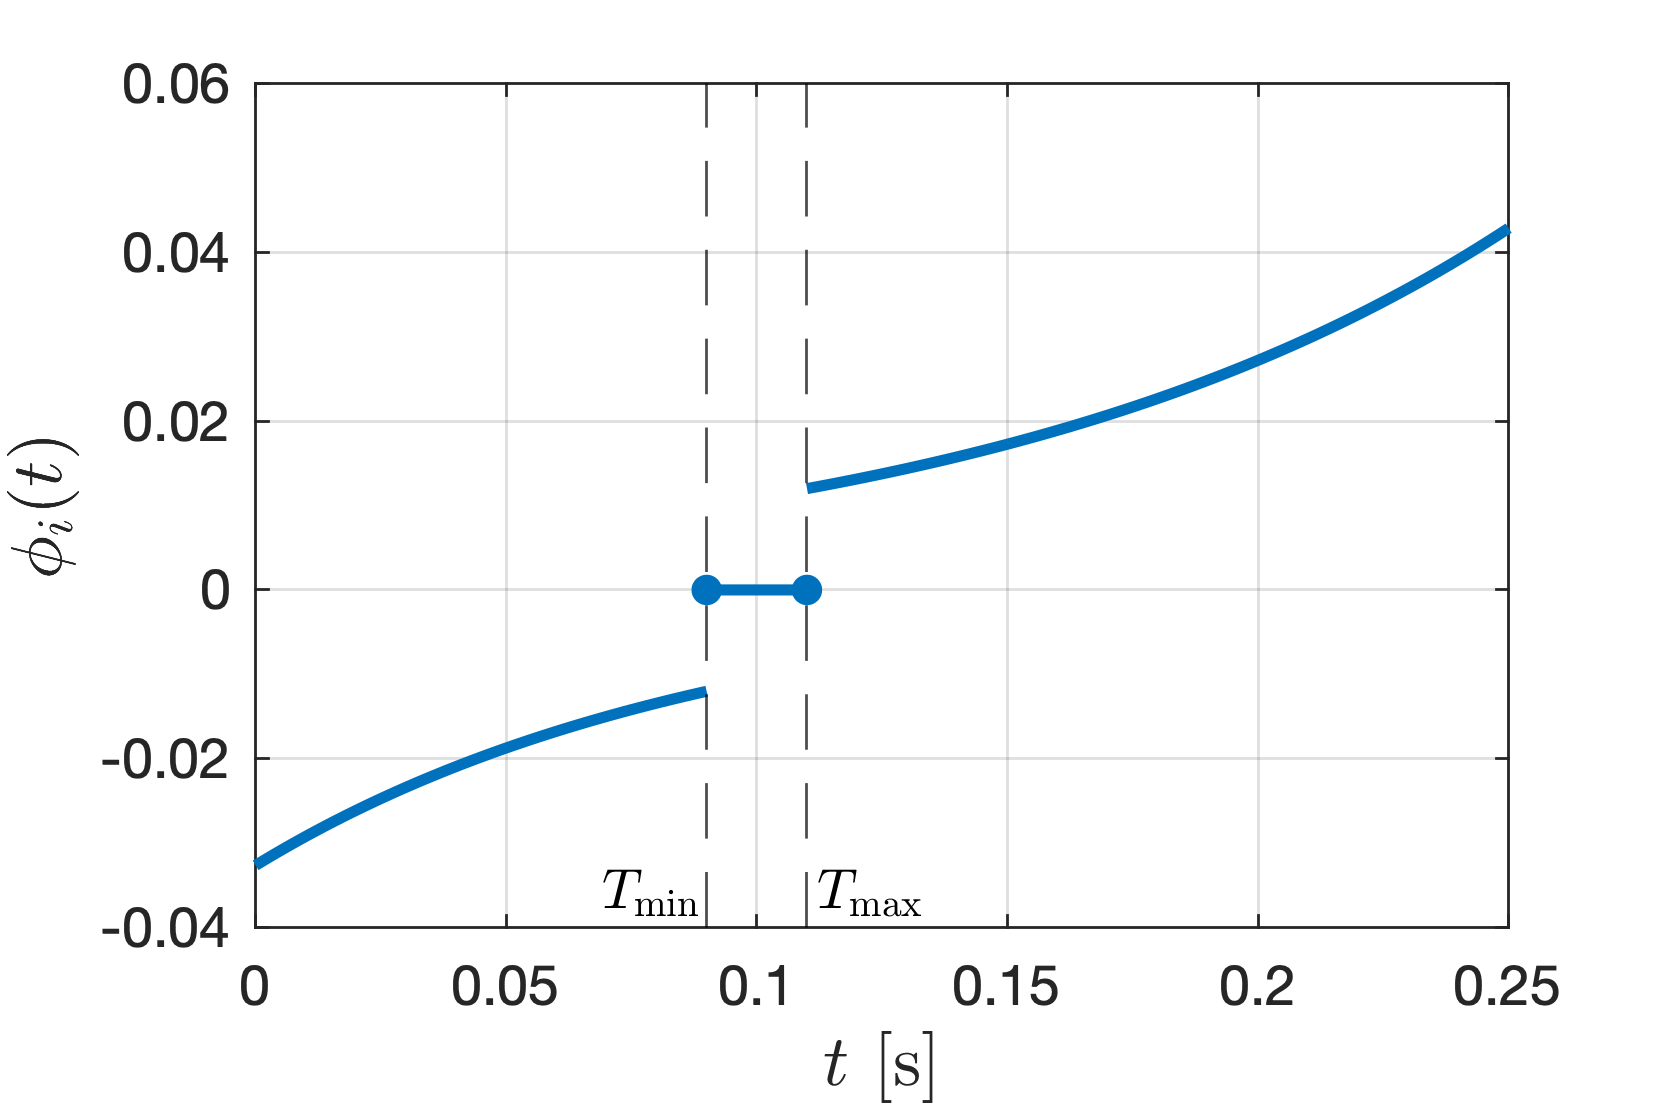
\includegraphics[width = 0.5\textwidth]{../Figures/IPlearningFunction.png}
\caption{The learning behaviour for the intrinsic plastiity.}
\label{fig:IPlearningFunction}
\end{figure}



\subsection{Custom learning windows}
Some of the behaviour we want to observe is currently not accounted for: synaptic strengths are unbounded and are generally nonzero. How can we model the behaviour where synaptic strengths can also settle on being zero? Perhaps a better idea than updating the synaptic strength by adding a new value, we can scale it.
\begin{itemize}
\item When $\Delta t_{ij}$ is very large (both positive and negative) we expect no change in the synaptic strength: $W(-\infty) = W(-\infty) = 0$. 
\item We expect a specific positive time delay to yield the most amount of synaptic strengthening: $\Delta t_{\rm best} = \underset{x}{\arg \max}  W(t)$
\item We expect small connections that have been reducing in size to quickly become zero, 
\item A better scaling system would be that not the out- or in-degree is constant, but 
\end{itemize}



\bibliographystyle{utphys}
\small{\bibliography{references}}

\label{LastPage}~

\end{document}
